\section{Sparsity}

We can use sparsity for image restoration. The idea behind this is, that a sparse signal is good for representing structure but not for white Gaussian noise. For this we model an image as follows:
$$\underbrace{y}_{\text{measured image}} = \underbrace{x}_{\text{original image}} + \underbrace{w}_{\text{noise}}$$

Now we perform MAP (maximum a posteriori) estimation:
$$E(x) = \frac{1}{2} ||y-x||_2^2 + \text{Pr}(x)$$

Where Pr is a log prior. Some classical priors to use would be smoothness ($\lambda || \mathcal L x||_2^2$ or total variation $\lambda ||\nabla x ||_1^2$. \medskip

Let $\mathbf D = [d_1, ..., d_p]$ be a set of normalized basis vectors, we call it \textbf{dictonary}. $\mathbf D$ is adapted to $x$ if it can represent it with few basic vectors, meaning a sparse vector $\alpha$ exists, so that $x \approx \mathbf D \alpha$. \medskip

There are predefined dictionaries, but we can also try to learn one ourself. We use the following model:
$$\min_{\alpha} \frac{1}{2} ||x - \mathbf D \alpha||_2^2 + \lambda \psi (\alpha)$$

Here $\psi$ induces sparsity and can be the $l_0, l_1, ...$ norm (we call it Lasso if $l_1$ is used). This idea can be expanded to not only perform denoising, but also do inpainting and demosaicking.


\section{Texture}

The key issues for textures are analysis / segmentation, representing the texture, and synthesis, generating textures.

\subsection{Representing Textures}

Textures are made up of stylised subelements, repeated in meaningful ways. To represent a texture we can try to find these subelements and represent their statistics. Finding the subelements can be done by applying filters and looking at the magnitude of the response. Possible filters could be spots and oriented bars at a variety of different scales (image pyramids).

\subsection{Texture Synthesis}

There is a variety of approaches to texture synthesis. One might use a histogram to capture the intensity probability distribution, but this does not capture any spatial relations. To improve on that one might use a co-occurrence matrix, having the probability distributions for intensity pairs. Other approaches are image-base, trying to perform "cut and paste". This is done by assuming Markov property and computing $P(p | N(p))$ ($N$ is the neighborhood of $p$).
\begin{center}
	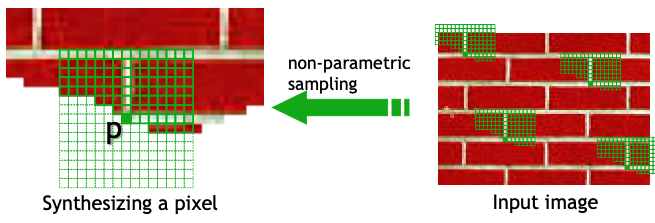
\includegraphics[width=\linewidth]{texture_syntezis.png}
\end{center}

To synthesize $p$, just pick one match at random. This can be expanded to work on patches of images and not single pixels.